\documentclass[11pt,a4paper]{article}
\usepackage{float}
\usepackage[utf8]{inputenc}
\usepackage[left=2cm,right=2cm,text={18cm,24cm},top=2cm]{geometry}
\usepackage[czech]{babel}
\usepackage{graphicx}
\usepackage{verbatim}
\usepackage{fancyvrb}
\usepackage{svg}
\usepackage{rotating}


\renewcommand{\familydefault}{\sfdefault}

\begin{document}
    \begin{titlepage}
        \begin{center}
            % FIT logo
            
\includegraphics[scale=0.65]{include/fit.pdf} \\

            \LARGE{
                \textbf{
                    Projektová dokumentace} \\
                Překladač jazyka IFJ22} \\
                
            \vspace{2cm}
            
            \Large{
                Tým xstrel03 \\
                Varianta TRP \\
            }
                
            \vspace{2cm}
            
            \normalsize{}
            \today{}

            \vspace{2cm}

            \begin{tabular}{l l l}
                \textbf{Matyáš Strelec} & \textbf{(xstrel03)}   & \quad X\% \\
                Ondřej Seidl            & (xseidl06)            & \quad X\% \\
                Maxmilián Nový          & (xnovym00)            & \quad X\% \\
                Dominik Klon            & (xklond00)            & \quad X\% \\
            \end{tabular}
        \end{center}
    \end{titlepage}

    \pagebreak{}

    \tableofcontents

    \pagebreak{}

    \section{Práce v týmu}
    Rozdělení práce mezi členy týmu (uveďte kdo a jak se podílel na jednotlivých
    částech projektu; povinně zdůvodněte odchylky od rovnoměrného rozdělení bodů).
    
    \subsection{Rozdělení práce}

    \subsection*{Matyáš Strelec}
    \begin{itemize}
        \item Lexikální analýza
        \item Syntaktická analýzy
        \item Dokumentace
    \end{itemize}

    \subsection*{Ondřej Seidl}
    \begin{itemize}
        \item Implementace tabulky symbolů
        \item Zpracování výrazů
    \end{itemize}

    \subsection*{Maxmilián Nový}
    \begin{itemize}
        \item Návrh LL-gramatiky
        \item Vestavěné funkce
    \end{itemize}

    \subsection*{Dominik Klon}
    \begin{itemize}
        \item Generování kódu
    \end{itemize}

    \subsection{Odchylky od rozvnoměrného rozdělení}
    

    \pagebreak{}

    \section{Lexikální analýza}

    \subsection{Datové struktury}
    Implementace lexikální analýzy je obsažena v souborech \verb|lexer.c| a \verb|lexer.h|.
    Pro potřeby lexikálního analyzátoru byly vytvořeny datové struktury které pomáhají při
    práci s tokeny a konečným automatem. Výčtový typ \verb|fsm_state_t| obsahuje všechny možné
    stavy konečného automatu dle návrhu, výčtový typ \verb|token_type_t| definuje typy tokenů.
    \\ \\
    Struktura \verb|token_t| obsahuje informace o tokenu, jeho typ, pozici v souboru, délku,
    a jeho předchůdce a následníka ve spojovém seznamu. Struktura \verb|token_list_t| obsahuje
    ukazatele na první, poslední, a aktuální token.

    \subsection{Funkce}

    Všechny funkce jsou ve zdrojových souborech popsané v komentářích, včetně jejich funkcionality, parametrů a návratových hodnot.
    \\ \\
    Funkce lexeru volaná z hlavního programu je funkce \verb|fillTokenList()|, která jako parametr
    dostává ukazatel na strukturu \verb|token_list_t|, kterou naplní seznamem tokenů pomocí volání
    funkce \verb|getNextToken()|. Funkce \verb|getNextToken()| je volána v cyklu, dokud není dosažen token
    typu konec souboru.
    \\ \\
    Funkce \verb|getNextToken()| je implementována pomocí konečného automatu. Dle posloupnosti znaků na vstupu
    určuje typ a vyplňuje data tokenu. V případě, že je na vstupu znak, který nelze podle automatu dále číst,
    je kontrolováno, jestli momentální stav automatu je koncový, pokud ano, token je validní.
    Dále jsou rozpoznána klíčová slova a odstraněny úvozovky z řetězců. Pokud automat není v koncovém stavu,
    ale na vstup přijde znak, který automat nemůže přečíst, funkce vrací chybu 1.
    \\ \\
    Dále soubor obsahuje funkce na práci se seznamem tokenů jako vázaným seznamem a funkce pro ladění.

    \subsection{Diagram konečného automatu}
    Vizte obrázek 1.
    
    \begin{figure}[H]
        \label{fig:FSM}
        \centering
        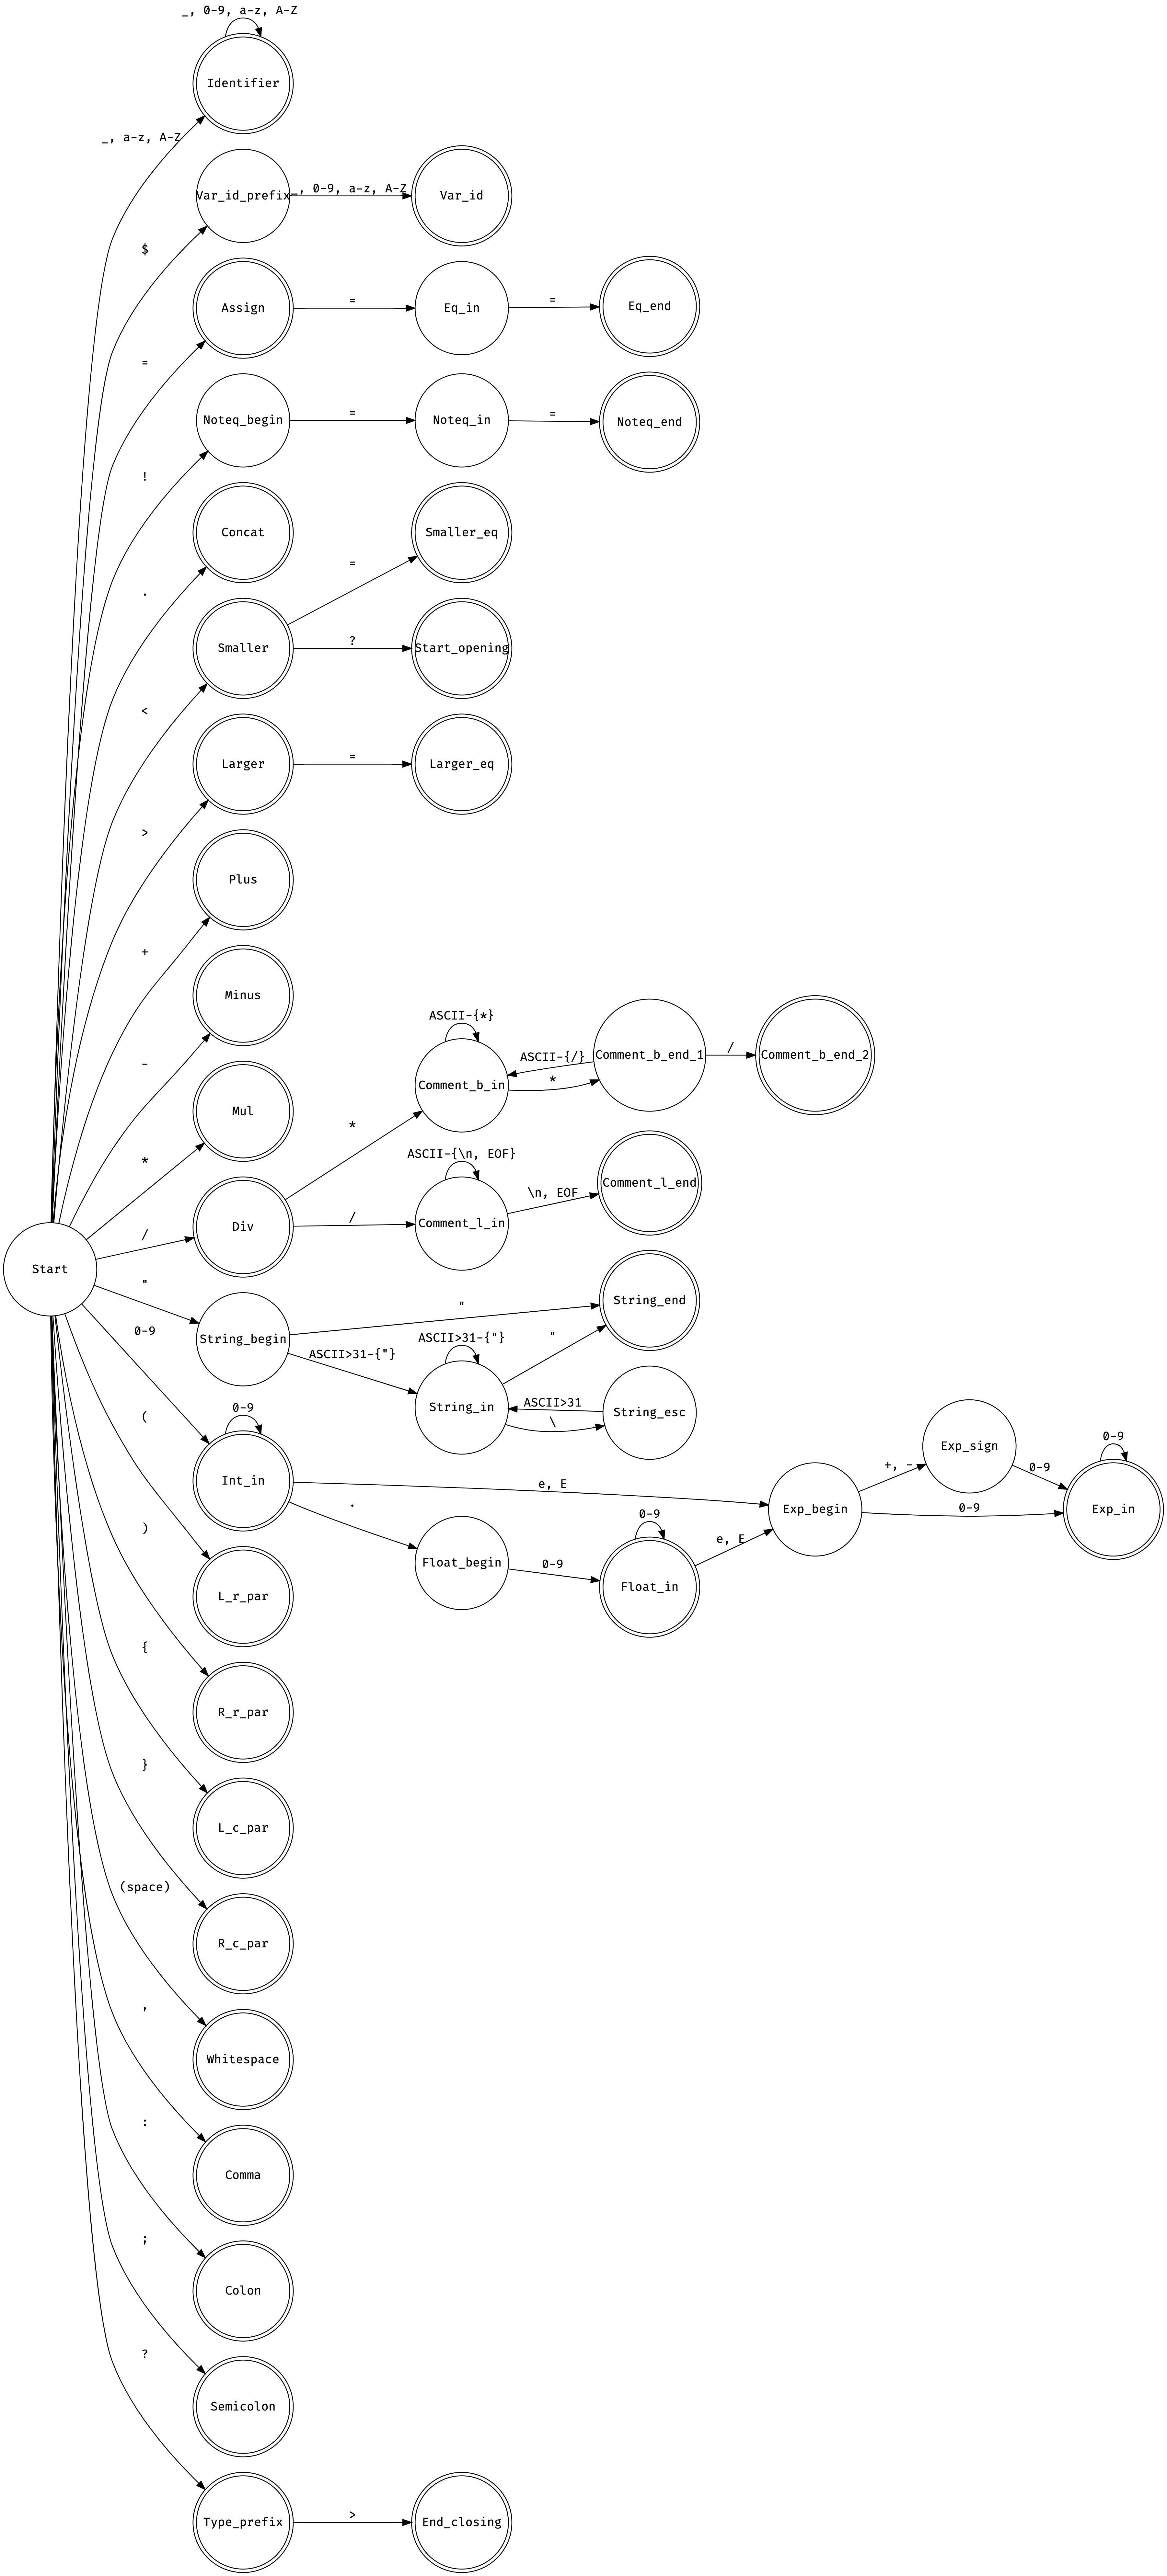
\includegraphics[height=0.97\textheight]{include/fsm.png}
        \caption{Diagram konečného automatu vytvořený nástrojem \texttt{Graphviz}}
    \end{figure}

    \pagebreak{}
    
    \section{Syntaktická analýza}
    
    \subsection{Implementace}

    \subsection{LL-gramatika}
    Pro jazyk IFJ22 byla navržena následující gramatika.
    \begin{Verbatim}
1:  <prog> -> <stat> <prog>
2:  <prog> -> function func-id ( <params> ) : type { <st-list> } <prog>
3:  <prog> -> <eof>

4:  <eof> -> ?> EOF
5:  <eof> -> EOF

6: <params-cont> -> , type $id <params-cont>
7: <params-cont> -> eps

8: <params> -> type $id <params-cont>
9: <params> -> eps

10: <args-cont> -> , <term> <args-cont>
11: <args-cont> -> 

12: <args> -> <term> <args-cont>
13: <args> -> eps

14: <stat> -> $id = <assign> ;
15: <stat> -> while ( <expr> ) { <st-list> }
16: <stat> -> if ( <expr> ) { <st-list> } else { <st-list> }
17: <stat> -> return <expr> ;
18: <stat> -> <expr> ;
19: <stat> -> func-id ( <args> ) ;

20: <st-list> -> <stat> <st-list>
21: <st-list> -> eps

22: <assign> -> <expr>
23: <assign> -> func-id ( <args> )

24: <term> -> $id
25: <term> -> val
    \end{Verbatim}
    \subsection*{Poznámky}
        \texttt{\$id} - identifikátor proměnné\\
        \texttt{func-id} - identifikátor funkce\\
        \texttt{val} - číselný nebo řetězcový literál \\
        \texttt{type} - datový typ (\texttt{int}, \texttt{double}, \texttt{string}) \\
        \texttt{func-id} - identifikátor funkce \\
        \texttt{eps} - $\varepsilon$ \\

    \subsection{LL-tabulka}

    \renewcommand{\familydefault}{\ttdefault}

    \begin{table}[h!]
        \begin{tabular}{|l|l|l|l|l|l|l|l|l|l|l|l|l|l|l|l|l|l|l|l|l|}
            \hline
                                             & \textbf{\begin{sideways}function   \ \end{sideways}}
                                                        & \textbf{\begin{sideways}func-id\end{sideways}}   
                                                                    & \textbf{\begin{sideways}(\end{sideways}}
                                                                            & \textbf{\begin{sideways})\end{sideways}}
                                                                                    & \textbf{\begin{sideways}:\end{sideways}}
                                                                                            & \textbf{\begin{sideways}type\end{sideways}}
                                                                                                    & \textbf{\begin{sideways}\{\end{sideways}}
                                                                                                            & \textbf{\begin{sideways}\}\end{sideways}}
                                                                                                                    & \textbf{\begin{sideways}?\textgreater{}\end{sideways}}
                                                                                                                                        & \textbf{\begin{sideways}EOF\end{sideways}}
                                                                                                                                                & \textbf{\begin{sideways},\end{sideways}}
                                                                                                                                                        & \textbf{\begin{sideways}\$id\end{sideways}}
                                                                                                                                                                & \textbf{\begin{sideways}=\end{sideways}}
                                                                                                                                                                    & \textbf{\begin{sideways}; \end{sideways}}
                                                                                                                                                                        & \textbf{\begin{sideways}while \end{sideways}}
                                                                                                                                                                                & \textbf{\begin{sideways}\textless{}expr\textgreater{}\end{sideways}}
                                                                                                                                                                                                                & \textbf{\begin{sideways}if\end{sideways}}
                                                                                                                                                                                                                        & \textbf{\begin{sideways}else\end{sideways}}
                                                                                                                                                                                                                                 & \textbf{\begin{sideways}return\end{sideways}}
                                                                                                                                                                                                                                            & \textbf{\begin{sideways}val\end{sideways}} \\ \hline
        \textbf{\textless{}prog\textgreater{}}        & 2        & 1         &       &       &      &        &       &       & 3                 & 3     &       & 1     &   &   & 1     & 1                             & 1     &        & 1        &         \\ \hline
        \textbf{\textless{}eof\textgreater{}}         &          &           &       &       &      &        &       &       & 4                 & 5     &       &       &   &   &       &                               &       &        &          &         \\ \hline
        \textbf{\textless{}params-cont\textgreater{}} &          &           &       & 7     &      &        &       &       &                   &       & 6     &       &   &   &       &                               &       &        &          &         \\ \hline
        \textbf{\textless{}params\textgreater{} }     &          &           &       & 9     &      & 8      &       &       &                   &       &       &       &   &   &       &                               &       &        &          &         \\ \hline
        \textbf{\textless{}args-cont\textgreater{}}   &          &           &       & 11    &      &        &       &       &                   &       & 10    &       &   &   &       &                               &       &        &          &         \\ \hline
        \textbf{\textless{}args\textgreater{} }       &          &           &       & 13    &      &        &       &       &                   &       &       & 12    &   &   &       &                               &       &        &          & 12      \\ \hline
        \textbf{\textless{}stat\textgreater{}  }      &          & 19        &       &       &      &        &       &       &                   &       &       & 14    &   &   & 15    & 18                            & 16    &        & 17       &         \\ \hline
        \textbf{\textless{}st-list\textgreater{}   }  &          & 20        &       &       &      &        &       & 21    &                   &       &       & 20    &   &   & 20    & 20                            & 20    &        & 20       &         \\ \hline
        \textbf{\textless{}assign\textgreater{}   }   &          & 23        &       &       &      &        &       &       &                   &       &       &       &   &   &       & 22                            &       &        &          &         \\ \hline
        \textbf{\textless{}term\textgreater{}    }    &          &           &       &       &      &        &       &       &                   &       &       & 24    &   &   &       &                               &       &        &          & 25      \\ \hline
    \end{tabular}
    \end{table}

    \subsection{Precedenční tabulka}
    \renewcommand{\familydefault}{\ttdefault}

    \begin{table}[h!]
        \begin{tabular}{|l|c|c|c|c|c|c|c|c|c|c|c|c|c|c|c|}
        \hline
                                 & \textbf{*}     & \textbf{/}     & \textbf{+}     & \textbf{-}     & \textbf{.}     & \textbf{\textless{}} & \textbf{\textgreater{}} & \textbf{\textless{}=} & \textbf{\textgreater{}=} & \textbf{===}   & \textbf{!==}   & \textbf{(}  & \textbf{)}     & \textbf{var} & \textbf{\$}    \\ \hline
        \textbf{*}               & \textgreater{} & \textgreater{} & \textgreater{} & \textgreater{} & \textgreater{} & \textgreater{}       & \textgreater{}          & \textgreater{}        & \textgreater{}           & \textgreater{} & \textgreater{} & \textless{} & \textgreater{} & \textless{}  & \textgreater{} \\ \hline
        \textbf{/}               & \textgreater{} & \textgreater{} & \textgreater{} & \textgreater{} & \textgreater{} & \textgreater{}       & \textgreater{}          & \textgreater{}        & \textgreater{}           & \textgreater{} & \textgreater{} & \textless{} & \textgreater{} & \textless{}  & \textgreater{} \\ \hline
        \textbf{+}               & \textless{}    & \textless{}    & \textgreater{} & \textgreater{} & \textgreater{} & \textgreater{}       & \textgreater{}          & \textgreater{}        & \textgreater{}           & \textgreater{} & \textgreater{} & \textless{} & \textgreater{} & \textless{}  & \textgreater{} \\ \hline
        \textbf{-}               & \textless{}    & \textless{}    & \textgreater{} & \textgreater{} & \textgreater{} & \textgreater{}       & \textgreater{}          & \textgreater{}        & \textgreater{}           & \textgreater{} & \textgreater{} & \textless{} & \textgreater{} & \textless{}  & \textgreater{} \\ \hline
        \textbf{.}               & \textless{}    & \textless{}    & \textgreater{} & \textgreater{} & \textgreater{} & \textgreater{}       & \textgreater{}          & \textgreater{}        & \textgreater{}           & \textgreater{} & \textgreater{} & \textless{} & \textgreater{} & \textless{}  & \textgreater{} \\ \hline
        \textbf{\textless{}}     & \textless{}    & \textless{}    & \textless{}    & \textless{}    & \textless{}    & \textgreater{}       & \textgreater{}          & \textgreater{}        & \textgreater{}           & \textgreater{} & \textgreater{} & \textless{} & \textgreater{} & \textless{}  & \textgreater{} \\ \hline
        \textbf{\textgreater{}}  & \textless{}    & \textless{}    & \textless{}    & \textless{}    & \textless{}    & \textgreater{}       & \textgreater{}          & \textgreater{}        & \textgreater{}           & \textgreater{} & \textgreater{} & \textless{} & \textgreater{} & \textless{}  & \textgreater{} \\ \hline
        \textbf{\textless{}=}    & \textless{}    & \textless{}    & \textless{}    & \textless{}    & \textless{}    & \textgreater{}       & \textgreater{}          & \textgreater{}        & \textgreater{}           & \textgreater{} & \textgreater{} & \textless{} & \textgreater{} & \textless{}  & \textgreater{} \\ \hline
        \textbf{\textgreater{}=} & \textless{}    & \textless{}    & \textless{}    & \textless{}    & \textless{}    & \textgreater{}       & \textgreater{}          & \textgreater{}        & \textgreater{}           & \textgreater{} & \textgreater{} & \textless{} & \textgreater{} & \textless{}  & \textgreater{} \\ \hline
        \textbf{===}             & \textless{}    & \textless{}    & \textless{}    & \textless{}    & \textless{}    & \textless{}          & \textless{}             & \textless{}           & \textless{}              & \textgreater{} & \textgreater{} & \textless{} & \textgreater{} & \textless{}  & \textgreater{} \\ \hline
        \textbf{!==}             & \textless{}    & \textless{}    & \textless{}    & \textless{}    & \textless{}    & \textless{}          & \textless{}             & \textless{}           & \textless{}              & \textgreater{} & \textgreater{} & \textless{} & \textgreater{} & \textless{}  & \textgreater{} \\ \hline
        \textbf{(}               & \textless{}    & \textless{}    & \textless{}    & \textless{}    & \textless{}    & \textless{}          & \textless{}             & \textless{}           & \textless{}              & \textless{}    & \textless{}    & \textless{} & =              & \textless{}  &                \\ \hline
        \textbf{)}               & \textgreater{} & \textgreater{} & \textgreater{} & \textgreater{} & \textgreater{} & \textgreater{}       & \textgreater{}          & \textgreater{}        & \textgreater{}           & \textgreater{} & \textgreater{} &             & \textgreater{} &              & \textgreater{} \\ \hline
        \textbf{var}             & \textgreater{} & \textgreater{} & \textgreater{} & \textgreater{} & \textgreater{} & \textgreater{}       & \textgreater{}          & \textgreater{}        & \textgreater{}           & \textgreater{} & \textgreater{} &             & \textgreater{} &              & \textgreater{} \\ \hline
        \textbf{\$}              & \textless{}    & \textless{}    & \textless{}    & \textless{}    & \textless{}    & \textless{}          & \textless{}             & \textless{}           & \textless{}              & \textless{}    & \textless{}    & \textless{} &                & \textless{}  &                \\ \hline
        \end{tabular}
        \end{table}
                        
        \renewcommand{\familydefault}{\sfdefault}

    \section{Sémantická analýza}


    \section{Tabulka symbolů}


    \section{Generování kódu}
    

    \section{Hlavní program}

\end{document}
